\section{Implementation}

\subsection{How to include figures}

\begin{figure}
		\centerline{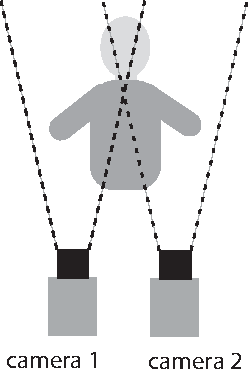
\includegraphics[width=0.20\textwidth]{fig}}		
		\caption{This is my first figure.}
		\label{fig:test}
\end{figure}

It is pretty easy to include figures in your document.  As a basic rule, let LaTeX place figures and tables.
Figure~\ref{fig:test} shows a simple example.
 	
\subsection{How to include tables}
	
	\begin{table}[h]
	\begin{center}	
		\begin{tabular}{|l|l|l|l|}
			
			\hline 
				% 1st line
				\textsc{Part 1} & 
				\textsc{Part 2} & 
				\textsc{Part 3} & 
				\textsc{Part 4}\\

				\hline 
				\hline 

				%2nd line
				test 1 &
				1 &
				2 &
				3 \\
				
				%3rd line
				test 2 &
				4 & 
				5&
				6 \\
				
				%4th line
				test 3 &
				7 &
				8 &
				9 \\

				\hline 
				
		\end{tabular}
	\caption{This is my first table.}
	\label{tab:test}
	\end{center}
	\end{table}	

Table~\ref{tab:test} presents a brief example of how to organize a table.  Every
table and figure should include a descriptive caption and should be referenced in the text.
	